\documentclass{beamer}
\usepackage[utf8]{inputenc}
\usepackage{MnSymbol}
\usepackage{qtree}
\usepackage{amssymb}
\usepackage{extarrows}
\usepackage{tikz}
\usepackage{mathrsfs}
\usetikzlibrary{arrows,automata}
\usepackage{graphicx}
\usepackage{hyperref}
\usepackage{subcaption,graphicx}
\usetheme{CambridgeUS}  %% Themenwahl
\beamertemplatenavigationsymbolsempty
%\useoutertheme{split}
%\useinnertheme{rectangles}

%\usecolortheme{beaver}

\title{Bildbasierte Navigation mit Neuronalen Netzen: Kolloquium}
\author{Jan Robert Rösler}
\date{\today}

\begin{document}
\maketitle

\frame{\tableofcontents}

\section{Technischer Hintergrund}

\frame{\tableofcontents[currentsection]}

\begin{frame} 
  \frametitle{Deep Learning} 

\begin{figure}
	\centering
	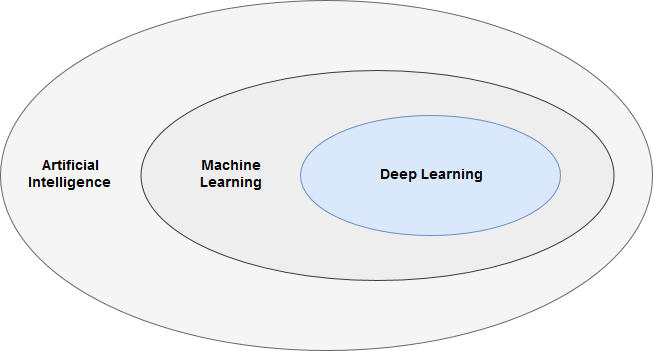
\includegraphics[width=.85\linewidth]{figures/Mengen.png}	 
	%\caption{}
	%Quelle: \protect\citeI{Architecture-ALVINN}
	\label{img:menge}
\end{figure}

\end{frame}

\begin{frame} 
\frametitle{Deep Learning} 


\end{frame}

\begin{frame}

\frametitle{Deep Learning mit Bildern}
\framesubtitle{Wie können Bilder in neuronalen Netzen verarbeitet werden?}

\begin{columns}[T]

\begin{column}[T]{5cm}
Möglich:\\
Matrix zu einem einspaltigen Inputvektor umwandeln.\newline

\textcolor{red}{Problem:}
\begin{itemize}
\item{\textcolor{red}{Räumliche Information geht verloren}}
\item{\textcolor{red}{Hoher Rechenaufwand}}
\end{itemize}

\end{column}

\begin{column}[T]{5cm}
	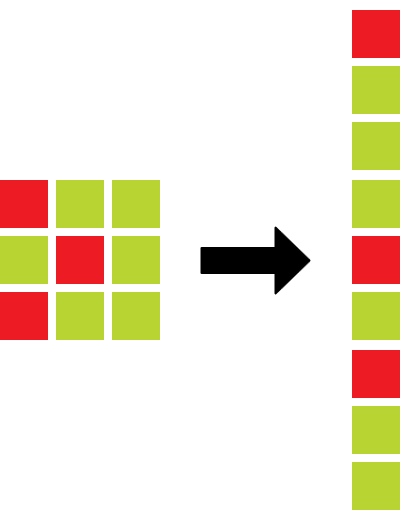
\includegraphics[scale=0.22]{figures/inputimage.png}	 
\end{column}

\end{columns}





\end{frame}

\begin{frame}
\frametitle{Convolutional Neural Network}

\end{frame}

\begin{frame}
\frametitle{Convolutional Neural Network 2}

\end{frame}

\begin{frame}
\frametitle{Vanishing Gradient Problem}

\end{frame}

\begin{frame}

\frametitle{Residual Networks}

\begin{columns}[T]

\begin{column}[T]{5cm}


\end{column}

\begin{column}[T]{5cm}
	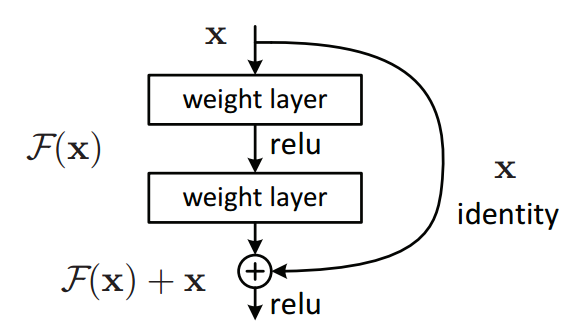
\includegraphics[scale=0.27]{figures/ResidualBlock.png}	 
\end{column}

\end{columns}

\end{frame}

\section{Idee}
\frame{\tableofcontents[currentsection]}

\begin{frame}
\frametitle{DroNet}
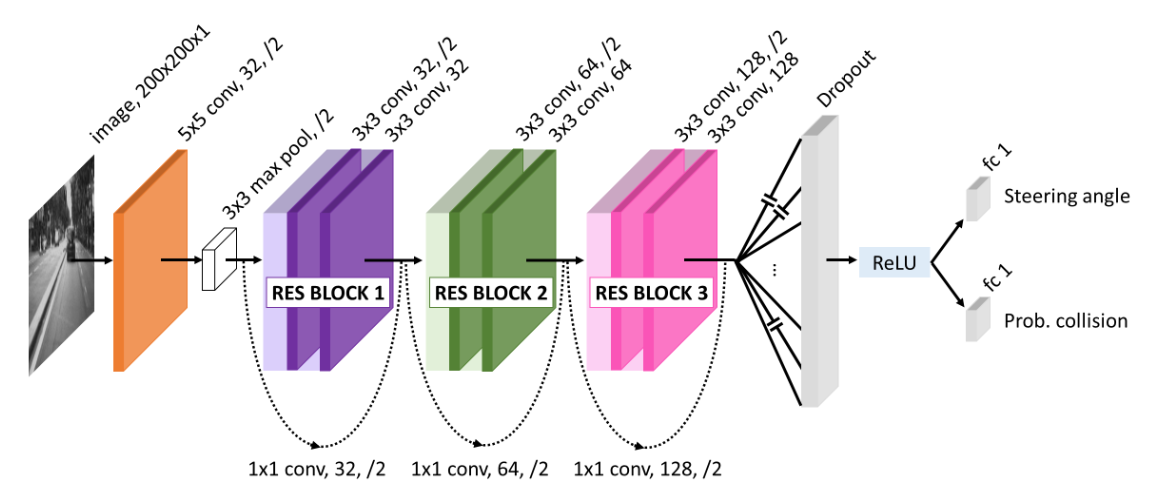
\includegraphics[width=\linewidth]{figures/Architecture-DRONET.png}	

\end{frame}

\begin{frame}
\frametitle{Ziel}

\end{frame}


\section{Entwurf}
\frame{\tableofcontents[currentsection]}

\begin{frame}
\frametitle{Bilder}

\begin{figure}
\centering
	\begin{subfigure}{.25\textwidth}
		  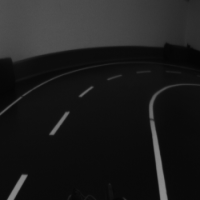
\includegraphics[scale=0.32]{figures/200x200.png}
	\end{subfigure}%
	\begin{subfigure}{.25\textwidth}
		  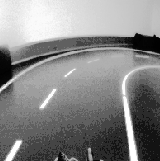
\includegraphics[scale=0.4]{figures/200x200Hist.png}
	\end{subfigure}%
	\begin{subfigure}{.25\textwidth}
		  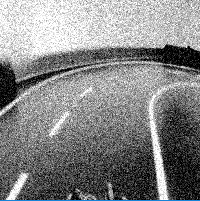
\includegraphics[scale=0.43]{figures/200x200Gauss.png}
	\end{subfigure}%
\end{figure}


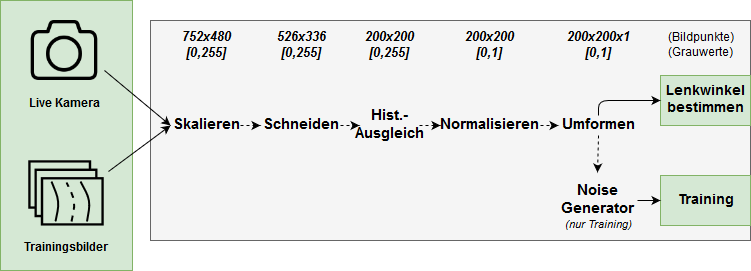
\includegraphics[width=\linewidth]{figures/Pipeline.png}	




\end{frame}

\begin{frame}
\frametitle{Traning}
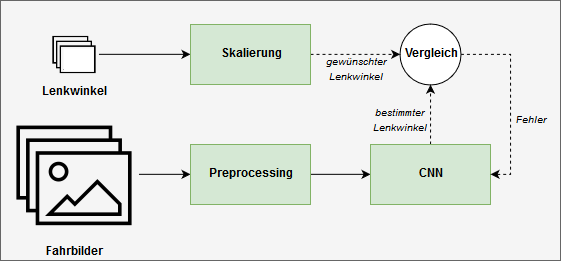
\includegraphics[width=\linewidth]{figures/Lernarchitektur.png}	 
\end{frame}

\begin{frame}
\frametitle{Steuerung}
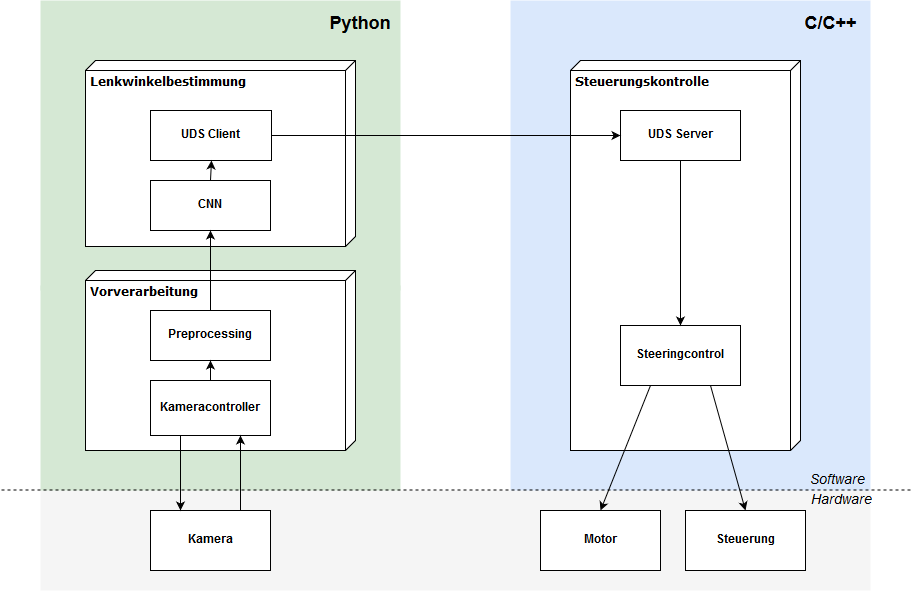
\includegraphics[width=\linewidth]{figures/Steuerung.png}	 

\end{frame}


\section{Ergebnis}
\frame{\tableofcontents[currentsection]}

\begin{frame}
\frametitle{Auswertung}
\framesubtitle{Training}

\end{frame}


\begin{frame}
\frametitle{Auswertung}
\framesubtitle{Testfahrt}

\centering
{\huge $\xrightarrow{}$} {\huge Aufnahmen} 

\end{frame}

\begin{frame}
\frametitle{Testfahrt}
\framesubtitle{Performance messen - Metrik}
\begin{equation}
Autonomiewert = (1 -  \frac{\text{Anzahl Fehler}\cdot 2 s}{\text{Fahrzeit in Sekunden}})\cdot 100
\end{equation}
\end{frame}

\begin{frame}
\frametitle{Testfahrt}
\framesubtitle{Performancemessung}

\begin{table}[h]
  \begin{center}
    \label{tab:testfahrten}
    \begin{tabular}{l|c|r} % <-- Alignments: 1st column left, 2nd middle and 3rd right, with vertical lines in between
      \textbf{Algorithmus} & \textbf{Fehler Runde 1} & \textbf{Fehler Runde 2}\\
      \hline
      DroNet & 16 & 12\\
      Carolo-Projekt & 7 & 11\\
       BA-RR& 3 & 5\\
    \end{tabular}
  \end{center}
\end{table}

\end{frame}

\begin{frame}
\frametitle{Testfahrt}
\framesubtitle{Performancevergleich}

\begin{table}[h]
  \begin{center}
    \label{tab:autonomie}
    \begin{tabular}{l|r}
      \textbf{Algorithmus} & \textbf{Autonomiewert} \\
      \hline
      DroNet & 53 \% \\
      Carolo-Projekt & 70 \%  \\
       BA-RR& 87 \% \\
    \end{tabular}
  \end{center}
\end{table}

\end{frame}

\begin{frame}
\frametitle{Auswertung}
\framesubtitle{Visualisierung}
Verschiedene Möglichkeiten

\end{frame}

\section{Schluss}
\frame{\tableofcontents[currentsection]}

\begin{frame}
\frametitle{Bewertung}

\end{frame}

\begin{frame}
\frametitle{Ausblick}

\end{frame}


\end{document}